% Created 2018-08-21 Tue 07:52
% Intended LaTeX compiler: pdflatex
\documentclass[a4paper]{article}
\usepackage[utf8]{inputenc}
\usepackage[T1]{fontenc}
\usepackage{graphicx}
\usepackage{grffile}
\usepackage{longtable}
\usepackage{wrapfig}
\usepackage{rotating}
\usepackage[normalem]{ulem}
\usepackage{amsmath}
\usepackage{textcomp}
\usepackage{amssymb}
\usepackage{capt-of}
\usepackage{hyperref}
\usepackage{minted}
\usepackage[margin=0.8in]{geometry}
\usepackage{amssymb,amsmath}
\usepackage{fancyhdr} %For headers and footers
\pagestyle{fancy} %For headers and footers
\usepackage{lastpage} %For getting page x of y
\usepackage{float} %Allows the figures to be positioned and formatted nicely
\floatstyle{boxed} %using this
\restylefloat{figure} %and this command
\usepackage{url} %Formatting of urls
\usepackage{minted}
\setminted{frame=single,framesep=10pt}
\chead{}
\rhead{\today}
\cfoot{}
\rfoot{\thepage\ of \pageref{LastPage}}
\author{Nathan Hughes (\href{mailto:nah31@aber.ac.uk}{nah31@aber.ac.uk})}
\date{\today}
\title{Usage Instructions for Micro-CT Plant Images}
\hypersetup{
 pdfauthor={Nathan Hughes (\href{mailto:nah31@aber.ac.uk}{nah31@aber.ac.uk})},
 pdftitle={Usage Instructions for Micro-CT Plant Images},
 pdfkeywords={},
 pdfsubject={},
 pdfcreator={Emacs 27.0.50 (Org mode 9.1.9)},
 pdflang={English}}
\begin{document}

\maketitle
\clearpage

\section{Releases}
\label{sec:org275c173}
This software works as a iteration-based release, adding new features and optimising and as such please refer to \href{https://github.com/NPPC-UK/microCT\_grain\_analyser/releases}{releases} for the latest stable version.

\section{Usage}
\label{sec:org596304a}
Usage of this software is straightforward. Inputting a directory, a voxel size and a minimum size of expected grain objects will output and write grain statistics and image to file.

\subsection{Setup variables}
\label{sec:orgaa54d83}
A brief setup of environment variables are required, this is an example:

\begin{minted}[frame=lines,linenos=true,fontfamily=DejaVuSans]{matlab}
voxelSize = 68.8; % or whatever micro-meter to voxel ratio was used in scanning
minimumGrainSize = 10000; % a minimum grain size of interest
structEleSize = 5; % a size of structuring element to use for morphological operations

% Every folder in CT-Scans folder and every ISQ file in them
directory = '/home/files/CT-Scans/*.ISQ';

% More optional parameters which change type of scanning
startFrom = 1;
endAt = 0;
watershed = true;
\end{minted}

\subsection{Optional Parameters}
\label{sec:org717a8a0}

\begin{itemize}
\item \texttt{startFrom} indicates file to start at from the directory indicated, almost always use '1'. It's useful for if processing fails partway through
\item \texttt{endAt} is where the process will stop, useful for if you'd only like to use a few scans for testing. Default is 0 and this will process everything
\item \texttt{watershed} will be a boolean value which will toggle if the more robust and strict watersheding is triggered - this will make processing take a lot longer and at times may over-segment. Generally only use if scans are failing to separate properly, or are particularly small (i.e. wild types / barley)
\end{itemize}

\subsubsection{N.B.}
\label{sec:org546d1a2}

Scanco has been known to alter the filenames for a reason known only Minerva would know.
So be on the lookout for:
\begin{minted}[frame=lines,linenos=true,fontfamily=DejaVuSans]{bash}
C0000123.ISQ;1
\end{minted}

To get around this I recommend running a script something like this (or a sed equivalent):

\begin{minted}[frame=lines,linenos=true,fontfamily=DejaVuSans]{python}
from glob import glob
from os import rename

[rename(f, f.replace(';','')) for f in glob('*.ISQ;1')]
\end{minted}

\subsection{Running}
\label{sec:org953f8e9}
Running the program is as simple as calling the processDirectory function.
\begin{minted}[frame=lines,linenos=true,fontfamily=DejaVuSans]{octave}
% Will process all files found by rdir function
processDirectory(directory, structEleSize, voxelSize, minimumGrainSize);
\end{minted}

\section{Files and Functions}
\label{sec:org5b82d92}

\subsection{cleanWheat}
\label{sec:orgb59e1a1}
cleanWheat is a function which takes as input a filename location on disk of an ISQ raw image, it processes it and outputs a binary 3D image and a greyscale 3D image which has been cleaned and segmented.
\subsection{countGrain}
\label{sec:org19cec71}
countGrain takes cleaned image data, separates each identified grain and computes statistics on a grain-per-grain basis. It returns two statistics objects, one with raw pixel data counted and another with computed metric values.
\subsection{filterSmallObjects}
\label{sec:org5deee47}
filterSmallObjects attempts to remove all objects which are smaller than the specified parameter during setup. This uses pixel size \textbf{not} metric sizes for this.
\subsection{imSurface}
\label{sec:orge23de4f}
imSurface is a library originally by David Legland. It measures the surface area in pixels of a 3D object.
\subsection{processDirectory}
\label{sec:org4f23add}
processDirectory is the main controlling function of this software, it moves image data around from function to function, gathers image results/measurements and saves it to disk from here.
\subsection{subdir}
\label{sec:org5f168da}
subdir is a function which recursively finds files, it is used to find files in sub-directories by using the '*' wildcard in the directory name parameter.
\begin{itemize}
\item This function was redone as the previous 'rdir' has operating issues with certain versions of windows.
\end{itemize}
\subsection{readISQ}
\label{sec:orgd126516}
readISQ originally developed by Johan Karlsson, we have modified it to make speed increases and added specific slice loading, this helps for increased speed when processing larger images
\subsection{segmentRachis}
\label{sec:org5d4a95c}
segmentRachis finds locations of nodes along the rachis of spikes of wheat, oats etc. Use of this data is primarily for locating joining points of split scans.
\subsection{watershed3D}
\label{sec:org8025ac3}
watershed3D incorporates traditional watershedding techniques and has adapted them to work in 3D. It also makes use of modernised distance-based watershed methods, by way of chessboard distance technique.
\subsection{writeTif}
\label{sec:orgba1736b}
writeTif writes image stacks to disk as TIF formatted files.


\section{Output}
\label{sec:org7bf3771}
From successful running of this software output will be:
\begin{itemize}
\item A statistics of grains CSV with metric values
\item A statistics of grains CSV with raw values
\item A TIF file of the segmented image
\item A statistics file of the rachis top and bottom points.
\item A folder of 2D cross sectional images, for each grain
\item A folder of 3D TIF files, each a individual grain
\end{itemize}

The output folder should look similar to this:

\begin{center}
\begin{center}
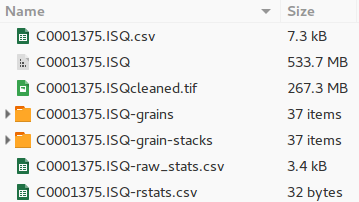
\includegraphics[width=.9\linewidth]{./directory.png}
\end{center}
\end{center}
\end{document}